\chapter{复立太子的曲折}
% 原书第63页

太子被废后，朝廷上下一致推举皇八子为新太子，但康熙拒绝这个提议，坚持要复立太子。纪理安记录中的大脉络与这段广为人知的历史进程相一致。从1708年12月开始，一直到来年4月，康熙与朝臣为新太子人选争执了四个月，经过数次尖锐的争吵，双方依然不能达成共识。纪理安的记载中提到群臣到最后都没有妥协，只是康熙找到了一个办法绕开众议来复立太子，这一点是传统史料中没有体现的部分。但就以往所知的材料来看，无论是朝鲜史料中记载的康熙在争论中“殴曳马齐”，还是清史中记载的马齐“拂袖而出”，都是对当时激烈争执的直观写照。双方在争论什么，分歧点又在哪里？要全面了解太子复立中的曲折，总结起来就是四个问题：


% 原书第63页

\begin{bookquote}一、康熙为什么想要复立太子？\end{bookquote}

% 原书第64页

\begin{bookquote}二、众人为什么会一致推举皇八子？\end{bookquote}

% 原书第64页

\begin{bookquote}三、康熙为什么不选皇八子？\end{bookquote}

% 原书第64页

\begin{bookquote}四、群臣为什么不愿意复立太子？\end{bookquote}
\section{康熙为什么想要复立太子？}

% 原书第64页

对于康熙为什么想要复立太子，以前史家的立足点是，康熙认为废黜太子引发了众皇子对储位的凯觎，因而借着“镇魇”这一巫术事件，用复立太子来结束储位之争。这种解释最大的问题是，在立论时其实心中已经知晓了后面数十年的储位之争，存有斗争很残酷这样的认识，因此猜想康熙想要赶快结束它。但实际上站在当时人的角度，康熙以及所有朝臣都不知道后面的事，没有人知道康熙能活多久，也没有人知道康熙复立了太子后会再度废黜。“储位争斗很残酷”这是一个很典型的后见之明，它让我们忽视了一个最简单最直白的原因：康熙要复立太子是认为自己真的错怪了太子。


% 原书第64–65页

现当代学者对这种最直接原因的忽视其实源于对两个问题认识不足：一是对镇魇等巫术在科学普及以前的社会中，之于个人决策的影响认知不足。二是对康熙与太子间的感情基础认识不够，也就是说在主观感情上，康熙是大大偏心太子的。


% 原书第65页

首先，对镇魇这样的巫术的认识需要放到当时的时代背景下理解。无论东方还是西方，在19世纪前，都没有现代的科学观。我们不能以今度古。对于历史来说，重要的不是我们现代人怎么认识巫术，而是当时的人怎么理解。就算是在18世纪前的西方社会也承认巫术的存在，而且认为诅咒、算命以及解除诅咒都是巫术的最基本形式。\NoteRef{03}{1}同样，镇魇、算命、驱魔也是明清社会生活的一部分，以至于明清律法中有专门的条例规定。明律中就有条文以“若造魇魅符书咒诅欲以杀人者，各以谋杀论”开头，规定了各种可能发生的情况。\NoteRef{03}{2}清律更为详细地规定了使用巫术或谋财或害命等各种情况的判罚。\NoteRef{03}{3}也就是说，当时社会是承认这些巫术的存在及其效果的，所以订立了专门的律例来惩罚。这和现代科学体系下对巫术的认识完全不一样。现代社会不相信巫术可能产生后果，因而也就没有了巫术相关的法律条款。


% 原书第65页

《红楼梦》第二十五回讲到赵姨娘请一位道婆使用镇魇之法来暗害贾宝玉和王熙凤，广为人知，其中的具体情节或可为了解清代社会中的镇魇作一参考：


% 原书第65–66页

\begin{bookquote}（道婆）掏出十个纸铰的青面白发的鬼来，并两个纸人，递与赵姨娘，又悄悄的教他道：“把他两个的年庚八字写在这两个纸人身上，一并五个鬼都掖在他们各人的床上就完了。我只在家里作法，自有效验。千万小心，不要害怕！”\end{bookquote}

% 原书第66页

\begin{bookquote}宝玉忽然“嗳哟”了一声，说：“好头疼！”林黛玉道：“该，阿弥陀佛！”只见宝玉大叫一声：“我要死！”将身一纵，离地跳有三四尺高，口内乱嚷乱叫，说起胡话来了。林黛玉并丫头们都唬慌了，忙去报知王夫人、贾母等。此时王子腾的夫人也在这里，都一齐来时，宝玉益发拿刀弄杖，寻死觅活的，闹得天翻地覆。贾母、王夫人见了，唬的抖衣乱颤，且“儿”一声“肉”一声放声恸哭。于是惊动诸人，连贾赦、邢夫人、贾珍、贾政、贾琏、贾蓉、贾芸、贾萍、薛姨妈、薛蟠并周瑞家的一干家中上上下下里里外外众媳妇丫头等，都来园内看视。登时园内乱麻一般。正没个主见，只见凤姐手持一把明晃晃钢刀砍进园来，见鸡杀鸡，见狗杀狗，见人就要杀人。众人越发慌了。周瑞媳妇忙带着几个有力量的胆壮的婆娘上去抱住，夺下刀来，抬回房去。平儿、丰儿等哭的泪天泪地。……\end{bookquote}

% 原书第66页

《红楼梦》是文学创作，同时也被公认为是当时社会现实的写照。正因为这一段镇魇的描写，从蔡元培开始便有一些红学学者猜测《红楼梦》中的人物与废太子及其子女有关。\NoteRef{03}{4}反倒是历史学者对镇魇以及镇魇后的症状没有给予足够正视。在《实录》中，康熙废太子后一周，尚未回到北京城时，就多次说到太子的各种症状：


% 原书第67页

\begin{bookquote}康熙四十七年九月十一日甲申（10月24日）：\end{bookquote}

% 原书第67页

\begin{bookquote}谕内大臣、大学士、翰林官员等：“近观允礽行事，与人大有不同，昼多沉睡，夜半方食，饮酒数十巨觥不醉。……居处失常，语言颠倒，竟类狂易之疾，似有鬼物凭之者。”\end{bookquote}

% 原书第67页

\begin{bookquote}康熙四十七年九月十五日戊子（10月28日）：\end{bookquote}

% 原书第67页

\begin{bookquote}谕大学士等：“允礽宫人所居撷芳殿，其地阴黯不洁，居者辄多病亡。允礽时常往来其间，致中邪魅，不自知觉。以此观之，种种举动，皆有鬼物使然。大是异事。”\end{bookquote}

% 原书第67页

\begin{bookquote}康熙四十七年九月十六日己丑，回京当天（10月29日）：\end{bookquote}

% 原书第67–68页

\begin{bookquote}大学士等遵旨……于午门内宣谕曰：“……今忽为鬼魅所凭，蔽其本性，忽起忽坐，言动失常。时见鬼魅，不安寝处，屡迁其居，啖饭七八碗尚不知饱，饮酒二三十觥亦不见醉。匪特此也，细加讯问，更有种种骇异之事……”\NoteRef{03}{5}\end{bookquote}

% 原书第68页

《实录》所载太子种种怪异举动，对比参照《红楼梦》对宝玉的描述，有很多相似之处。而且这里需要注意，康熙描述太子的这些异常举动是在发现大皇子镇魇案前一个多月。在正视了太子的异常后，再来重看关于李光地的记录：


% 原书第68页

\begin{bookquote}还宫有顷，（康熙）召公（注：李光地）独对。公顿首请曰：“帐殿之警，上果稔知其主名？必无剌谬乎？”上默不答，怅然久之，曰：“此直为鬼物所戏耳，何丧心至是？”\end{bookquote}

% 原书第68页

也就是说康熙从一开始就有“鬼物”的怀疑。康熙这段单独谈话是他刚回到北京时和李光地进行的。


% 原书第68–69页

康熙身为父亲，一旦怀疑是有“鬼物”作祟，便采取过行动，上文所引10月28日条目下，就记录了他命人查看“撷芳殿”，发现“其地阴黯不洁”。他希望找到太子问题的病根。康熙的言和行都反映出他确实怀疑过“鬼物”。只有明白了康熙确实怀疑过“鬼物”，才能理解当他一个月后得知大皇子设镇魇暗害太子，且亲眼看到了地下挖出来的人偶后，就会真心相信之前太子的种种异动是由于被“鬼物所戏”。镇魇之事不是康熙找到的借口，而是真正让康熙认为错怪了太子。也只有明白了这一点，才能理解本书前言所写的康熙父子二人见面后相顾无语流泪的场景。那次见面就在发现人偶的第二天。


% 原书第69–70页

要完全理解康熙的心情，其实还有必要了解一下康熙对太子的感情。康熙儿子众多，除去早夭的，获得排序名分的共二十四位，皇二十四子出生在1716年，也就是康熙六十三岁的时候。\NoteRef{03}{6}但在所有这些皇子中，二阿哥允礽在康熙心中的地位，是独一无二的。允礽出生在1674年，康熙时年二十一。第二年，允礽就被封为了太子。康熙对太子的特别钟爱和他年少时的经历密切相关。1661年，顺治驾崩，年仅八岁的康熙继位，两年后，其母也病逝了。年少的康熙虽贵为皇帝，但实际上是个孤儿。他在鳌拜等辅政大臣的控制下长大，童年缺少亲情，也缺乏安全感。宫里内廷外廷，包括身边侍卫，有很多都不是他能真正信任的人。登基六十年庆典时，叱咤风云、戎马一生的康熙当着群臣的面发出感慨：“父母膝下，未得一日承欢，此朕六十年来抱歉之处。”\NoteRef{03}{7}在康熙少年时代，有三位他既信任又能帮他的女人：一是他的奶奶孝庄太皇太后。二是顺治皇帝的第二位皇后，后来被称作孝惠章皇后（1641—1718），康熙的嫡母；相比于著名的孝庄太皇太后，康熙的嫡母在历史中存在感不强，但这位孝惠章皇后一直在宫里有很大的影响，康熙南巡或外出，都要派遣皇子定期问安。\NoteRef{03}{8}第三位就是太子的母亲，即康熙的第一位皇后孝诚仁皇后。孝诚仁皇后比康熙大三个月。两人1665年成婚时，双方按虚岁算都只有十二岁。这桩婚事遭到了鳌拜的反对，但还是在孝庄太皇太后的坚持下举行了。孝诚仁皇后是索尼长子噶布喇的女儿，而噶布喇又是宫中侍卫的统领之一。孝诚仁皇后和他的父亲由此成为康熙早年在宫里的依靠。索尼家族是满人贵族中少有的书香门第，一家上下都有很高的文化水平。这桩婚事把当时的四大辅臣之一的索尼及其家族变成了康熙的坚实后盾，成为他后来1669年扳倒鳌拜的靠山之一。对于康熙来说，孝诚仁皇后是一位与他年龄相仿的女子，在青少年时期便进入他的世界，并陪伴他度过了与鳌拜周旋的艰难岁月。康熙八年（1669）十二月，也就是康熙扳倒鳌拜的这一年年底，孝诚仁皇后生下了他们的第一个儿子。但这位皇子三年后不幸夭折。出生于1674年的允礽，是他们的第二个儿子。孝诚仁皇后在生下允礽后两个时辰就去世了。


% 原书第70–71页

传统的清史资料不会记载皇帝的私人感情，但一些细节颇能侧面反映。孝诚仁皇后去世后三天，棺木移放到紫禁城西侧。康熙一连二十一天，每天都要到停放棺材的地方追忆祭祀。之后，他更亲自护送灵柩到北京北郊的巩华城（今北京市昌平区沙河镇，距离故宫直线距离约三十五公里）中停放。但康熙不忍离开，一直守在灵柩旁，直到夜晚戌时（晚上7—9点）才起驾回宫。而接下来的六个月中，康熙去了三十四次巩华城（约每周都去）。据记载，康熙于康熙十六年（1677，孝诚仁皇后去世后三年）五月初二日巳时去往巩华城，在那里待到五月初三日巳时才离开。允礽出生的准确时间是康熙十三年五月初三日巳时，也就是说，康熙为了追忆祭奠孝诚仁皇后，细心到连时辰都精确安排过。据学者杨珍统计，三年之中，康熙共去过巩华城八十次。而这一时期，历史上三藩之乱（1673—1681）刚刚开始，正是康熙朝政忙碌之时。康熙这样频繁去往巩华城，甚至让朝鲜使节都感到不可思议，说康熙“不恤国事”，因为其经常去“往哭”故人。\NoteRef{03}{9}康熙与太子的母亲是有真感情的。


% 原书第71页

允礽在出生满周岁后就被立为太子，也是康熙对孝诚仁皇后感情的一个反映。立太子时，康熙实岁才满二十，而且满人本来也没有立太子的习俗，之前的顺治、皇太极、努尔哈赤都没有立过太子。此外，孝庄太皇太后也中意孝诚仁皇后，是立太子的支持者。了解了以上背景，才会明白为什么康熙决定复立太子后，会在朝堂上对大臣讲他的“故人”在给他托梦：


% 原书第71页

\begin{bookquote}近日有皇太子事，梦中见太皇太后，颜色殊不乐，但隔远默坐，与平时不同。皇后亦以皇太子被冤见梦。\NoteRef{03}{10}\end{bookquote}

% 原书第71页

从心理上说，康熙废黜太子后，觉得最对不起的人就是这两位，所以才会梦到她们。除了已去世的这两位，当时还活着的孝惠章皇后也是太子的支持者。\NoteRef{03}{11}所以从个人感情上来讲，康熙早年生命中对他影响最重要的三位女性都是太子的支持者。


% 原书第72页

康熙在立了太子后，对太子的教育也倾注了心血。他曾说过：“当允礽幼时，朕亲教以诗书。”\NoteRef{03}{12}允礽由于一生下来母亲就去世了，康熙在他身上花了很多精力。这是他们父子感情超过其他皇子的重要原因。康熙的皇子众多，皇孙就更多了，因而被皇帝亲自带过，对皇子皇孙来说是极高的殊荣。乾隆登基后就经常炫耀他是被康熙亲自带过的孙子。从父子感情上来说，尽管后来太子再度被废，但康熙给太子的待遇一直没变，也关心他的生活。二废太子后，康熙曾给大臣说：“朕与二阿哥并无间隔，即拘禁处，朕常遣内监往视，赐物赐食。”有一年夏天，他吩咐太监：“酸樱桃初得，色味俱佳，其大非常，比京中者悬绝远了。选大者，二阿哥处也送去。”\NoteRef{03}{13}


% 原书第72–73页

康熙与太子之间的感情是他迫不及待要在镇魇案后复立太子的重要原因。镇魇案还破除了康熙心中一直存在的一个疑虑，就是康熙一直担心他会在这一年里被加害。大皇子用镇魇加害了他，算是应验了他的预测，由此也就破除了他的疑虑。康熙有这个预测，跟当时满汉权贵相信算命，特别是八字测算有关。10月22日，也就是在行营宣布废黜太子五天后，康熙曾经对着身边的人说过：


% 原书第73页

\begin{bookquote}今岁有事，朕已预知。朕意中时若有一事将发者，曾向允礽（注：太子）言之。今岁朱三、一念和尚事发后，允礽奏曰：“皇父之言验矣。”朕谓之曰：“尚恐未尽于此也。”彼时亦不知所发何事，而不意竟有此事也。\NoteRef{03}{14}\end{bookquote}

% 原书第73页

“今岁有事，朕已预知”这段，以前也有学者注意到，可惜只是从心理学角度出发，认为这是康熙在“抑郁情绪”中的发言。\NoteRef{03}{15}但如果看过一些中国古代算命的书，就知道这段对话的场景，其实在测算书中是经常出现的固定模式。康熙经过测算，预先知道今年有事要发生，而且他还给太子讲过。当朱三、一念和尚这起谋反性质的事发生后，太子认为这件事就是康熙预测的事。但康熙答复说“尚恐未尽于此也”，也就是说康熙认为不止是这件事。就像有一个算命的人在年初给某人讲，今年你有血光之灾，那么当这人出了车祸，从医院治疗后出来，去问算命的人，你说的血光之灾就是这车祸吧？算命的人这时可能说，就是这事，但也有可能和康熙说的话一样：“尚恐未尽于此也。”而康熙说“不意竟有此事”，表示他认为之前的预测应验在了废黜太子这件事上。也就是这时他认为此前算到的“有事发生”已经应验了。


% 原书第74页

\begin{figure}[htbp]\centering
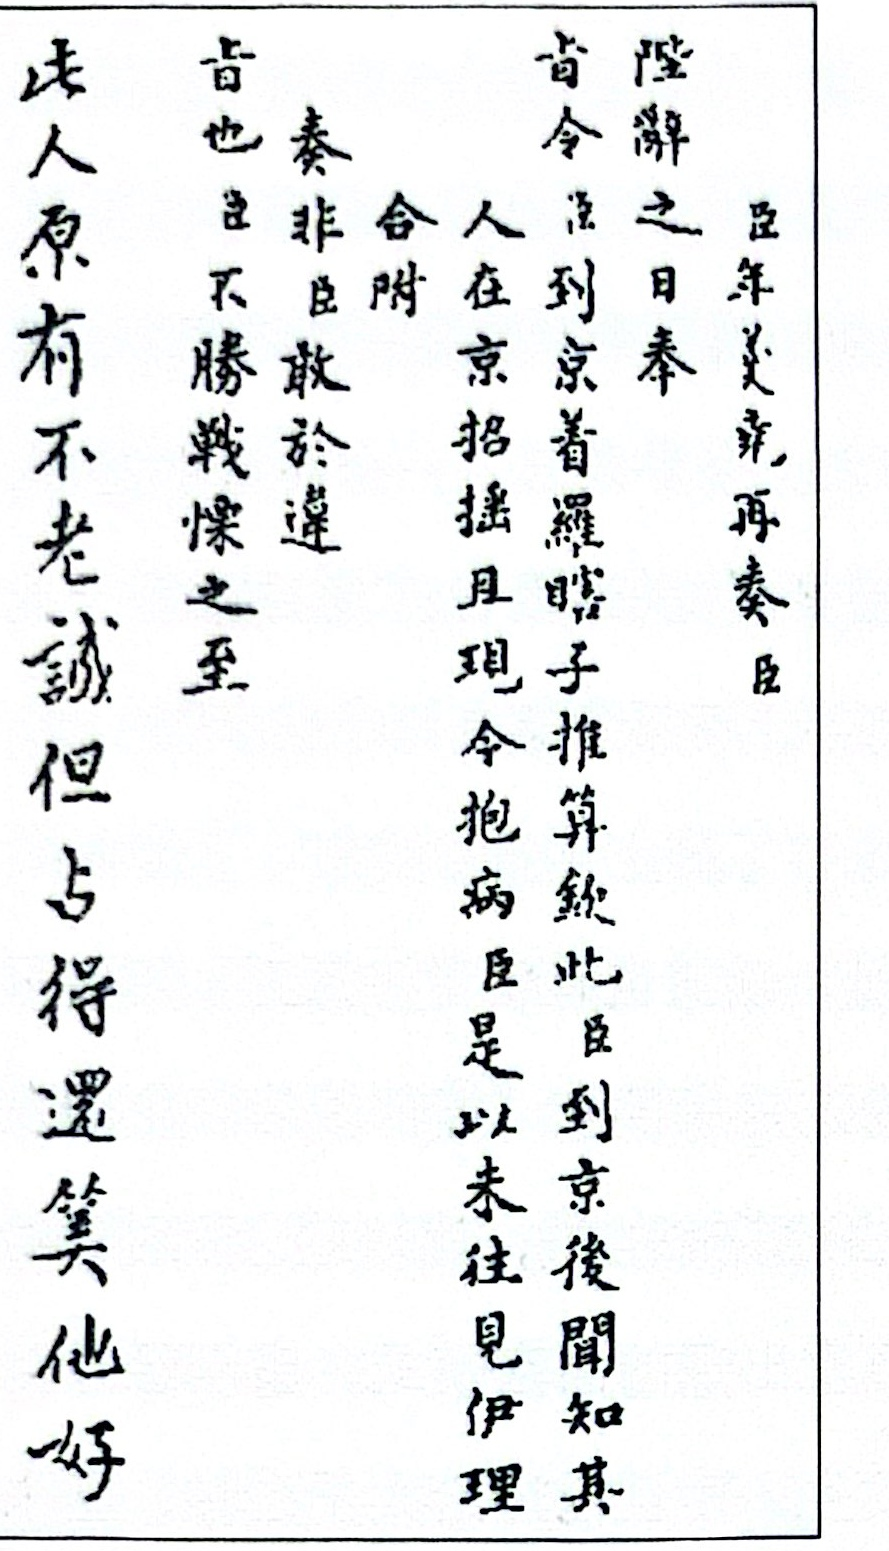
\includegraphics[width=.9\linewidth,height=.68\textheight,keepaspectratio]{assets/fig-96.jpg}
\caption{年羹尧上奏折解释未遵旨占卜之缘由及康熙朱批}\label{fig:96}\end{figure}


% 原书第74页

现存清史档案中，可以看到康熙一家都相信八字算命，康熙、皇十四子，以及雍正都留有八字算命的记录。比如，有一次已经是川陕总督的年羹尧到行宫拜见康熙后，康熙分派他去山西和陕西赈灾。年羹尧回到北京与官员交接，做了各种安排后，给康熙上了一道奏折汇报公务，同时他还附上了一份奏折告诉康熙（见图片\ref{fig:96}）：

% 原书第74页

\begin{bookquote}臣年羹尧再奏：臣陛辞之日奉旨，令臣到京，着罗瞎子推算。钦此。臣到京后闻知其人在京招摇，且现今抱病，臣是以未往见伊。理合附奏，非臣敢于违旨也。臣不胜战栗之至。\end{bookquote}

% 原书第74页

\begin{bookquote}（朱批）此人原有不老诚，但占得还算他好。\end{bookquote}

% 原书第74–75页

这里可以看到康熙不仅相信算命，还在见封疆大吏时，命其去测算，并且连找谁算都推荐了。年羹尧似乎对这个算命的人颇有微词，说其“在京招摇”。\NoteRef{03}{16}康熙承认这一点，但同时肯定此人的占算技术。一般瞎子用到的算命术就是测生辰八字，这也是当时皇家经常用到的方法，在清初的奏折中经常能见到。（见图片\ref{fig:98}、图片\ref{fig:99}、图片\ref{fig:100}）


% 原书第75页

康熙的生辰八字史料中没有明确记录。根据顺治朝《实录》，康熙出生在顺治十一年甲午三月十八日戊申（换算成公元纪年是1654年5月4日），但时辰就笔者所见资料尚不能确知。\NoteRef{03}{17}因而最后八字中表示时辰的两字用××代替：


% 原书第75页

\begin{center}
\renewcommand{\arraystretch}{1.25}
\begin{tabular}{|c|c|c|c|}
\hline
年 & 月 & 日 & 时 \\
\hline
甲午 & 戊辰 & 戊申 & ×× \\
\hline
\end{tabular}
\end{center}

% 原书第75页、第80页

所谓八字算命，就是把一个人出生时阴历的年、月、日、时辰，按照历法的规则分别对应一个干支，共八个字。比如1654年对应是甲午，三月对应是戊辰。“甲午”这两个字在一起称为干支，其中甲为天干，而午为地支。天干总共有十个：甲、乙、丙、丁、戊、己、庚、辛、壬、癸。地支有十二个：子、丑、寅、卯、辰、巳、午、未、申、酉、戌、亥。天干和地支根据阴阳配对，可以排列出六十种组合，就是我们常说的六十甲子。上面提到的甲午、戊辰都是六十甲子之一。人一出生，年、月、日、时就已经定下来了，也就是说八字就定下来了。这八字就是所谓一个人的命。算某一年的运程在算命中称为算流年。我们经常听说的“流年不利”，就是指这一年的运程不大好。\NoteRef{03}{18}康熙废太子的1708年，是戊子年。也就是康熙的八字在1708年遇到的是“戊子流年”。


% 原书第76页

\begin{figure}[htbp]\centering
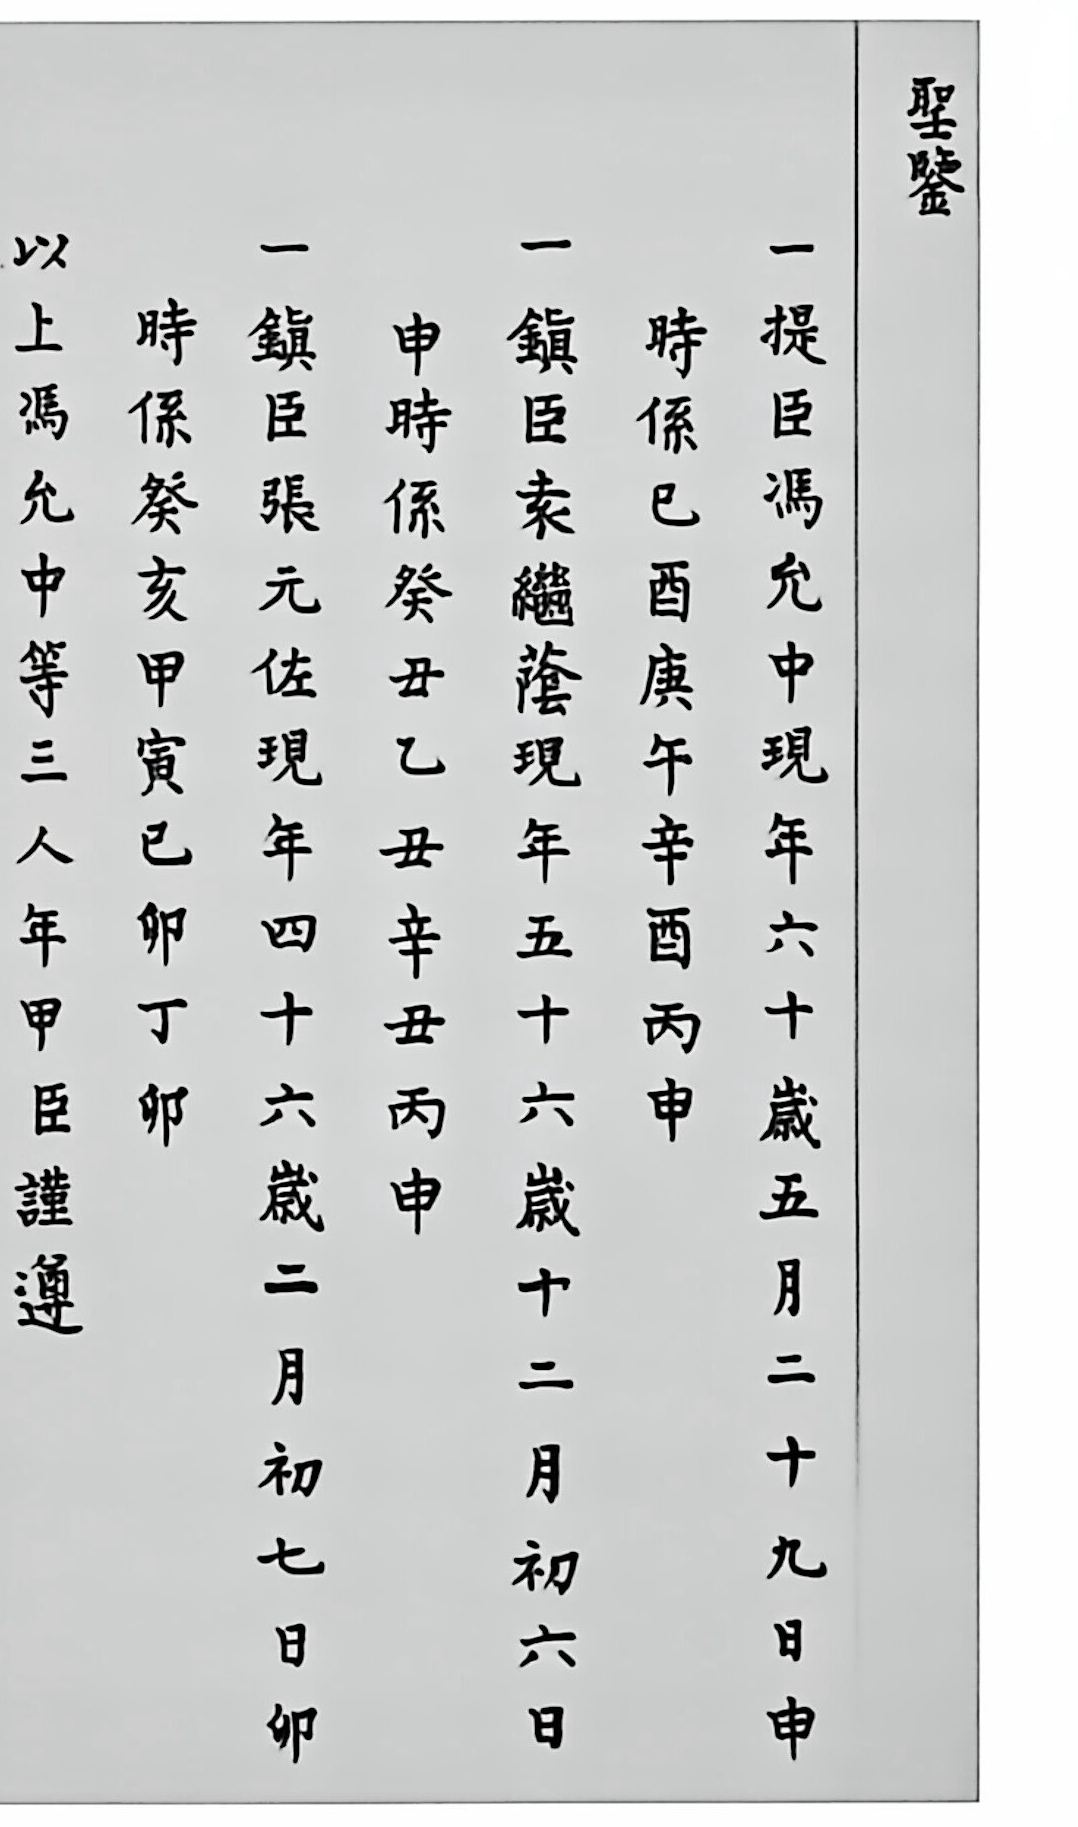
\includegraphics[width=.9\linewidth,height=.68\textheight,keepaspectratio]{assets/fig-98.jpg}
\caption{岳锺琪奏报官员生辰八字（台北故宫博物院清代档案检索系统，故宫003703号）}\label{fig:98}\end{figure}


% 原书第77页

\begin{figure}[htbp]\centering
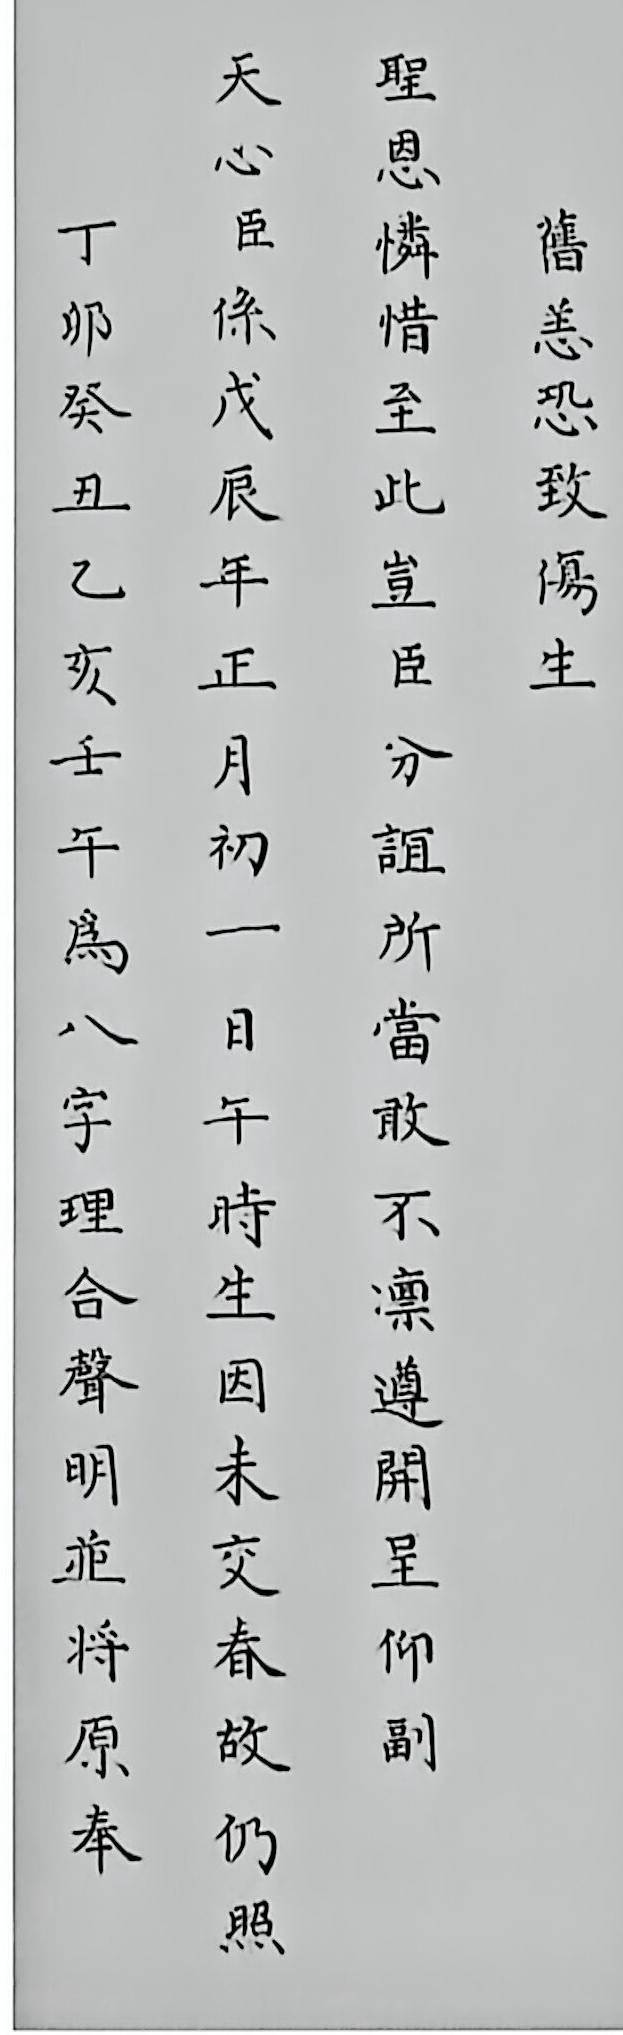
\includegraphics[width=.9\linewidth,height=.68\textheight,keepaspectratio]{assets/fig-99.jpg}
\caption{李卫上报生辰八字（台北故宫博物院清代档案检索系统，故宫010751号）}\label{fig:99}\end{figure}


% 原书第78页

\begin{figure}[htbp]\centering
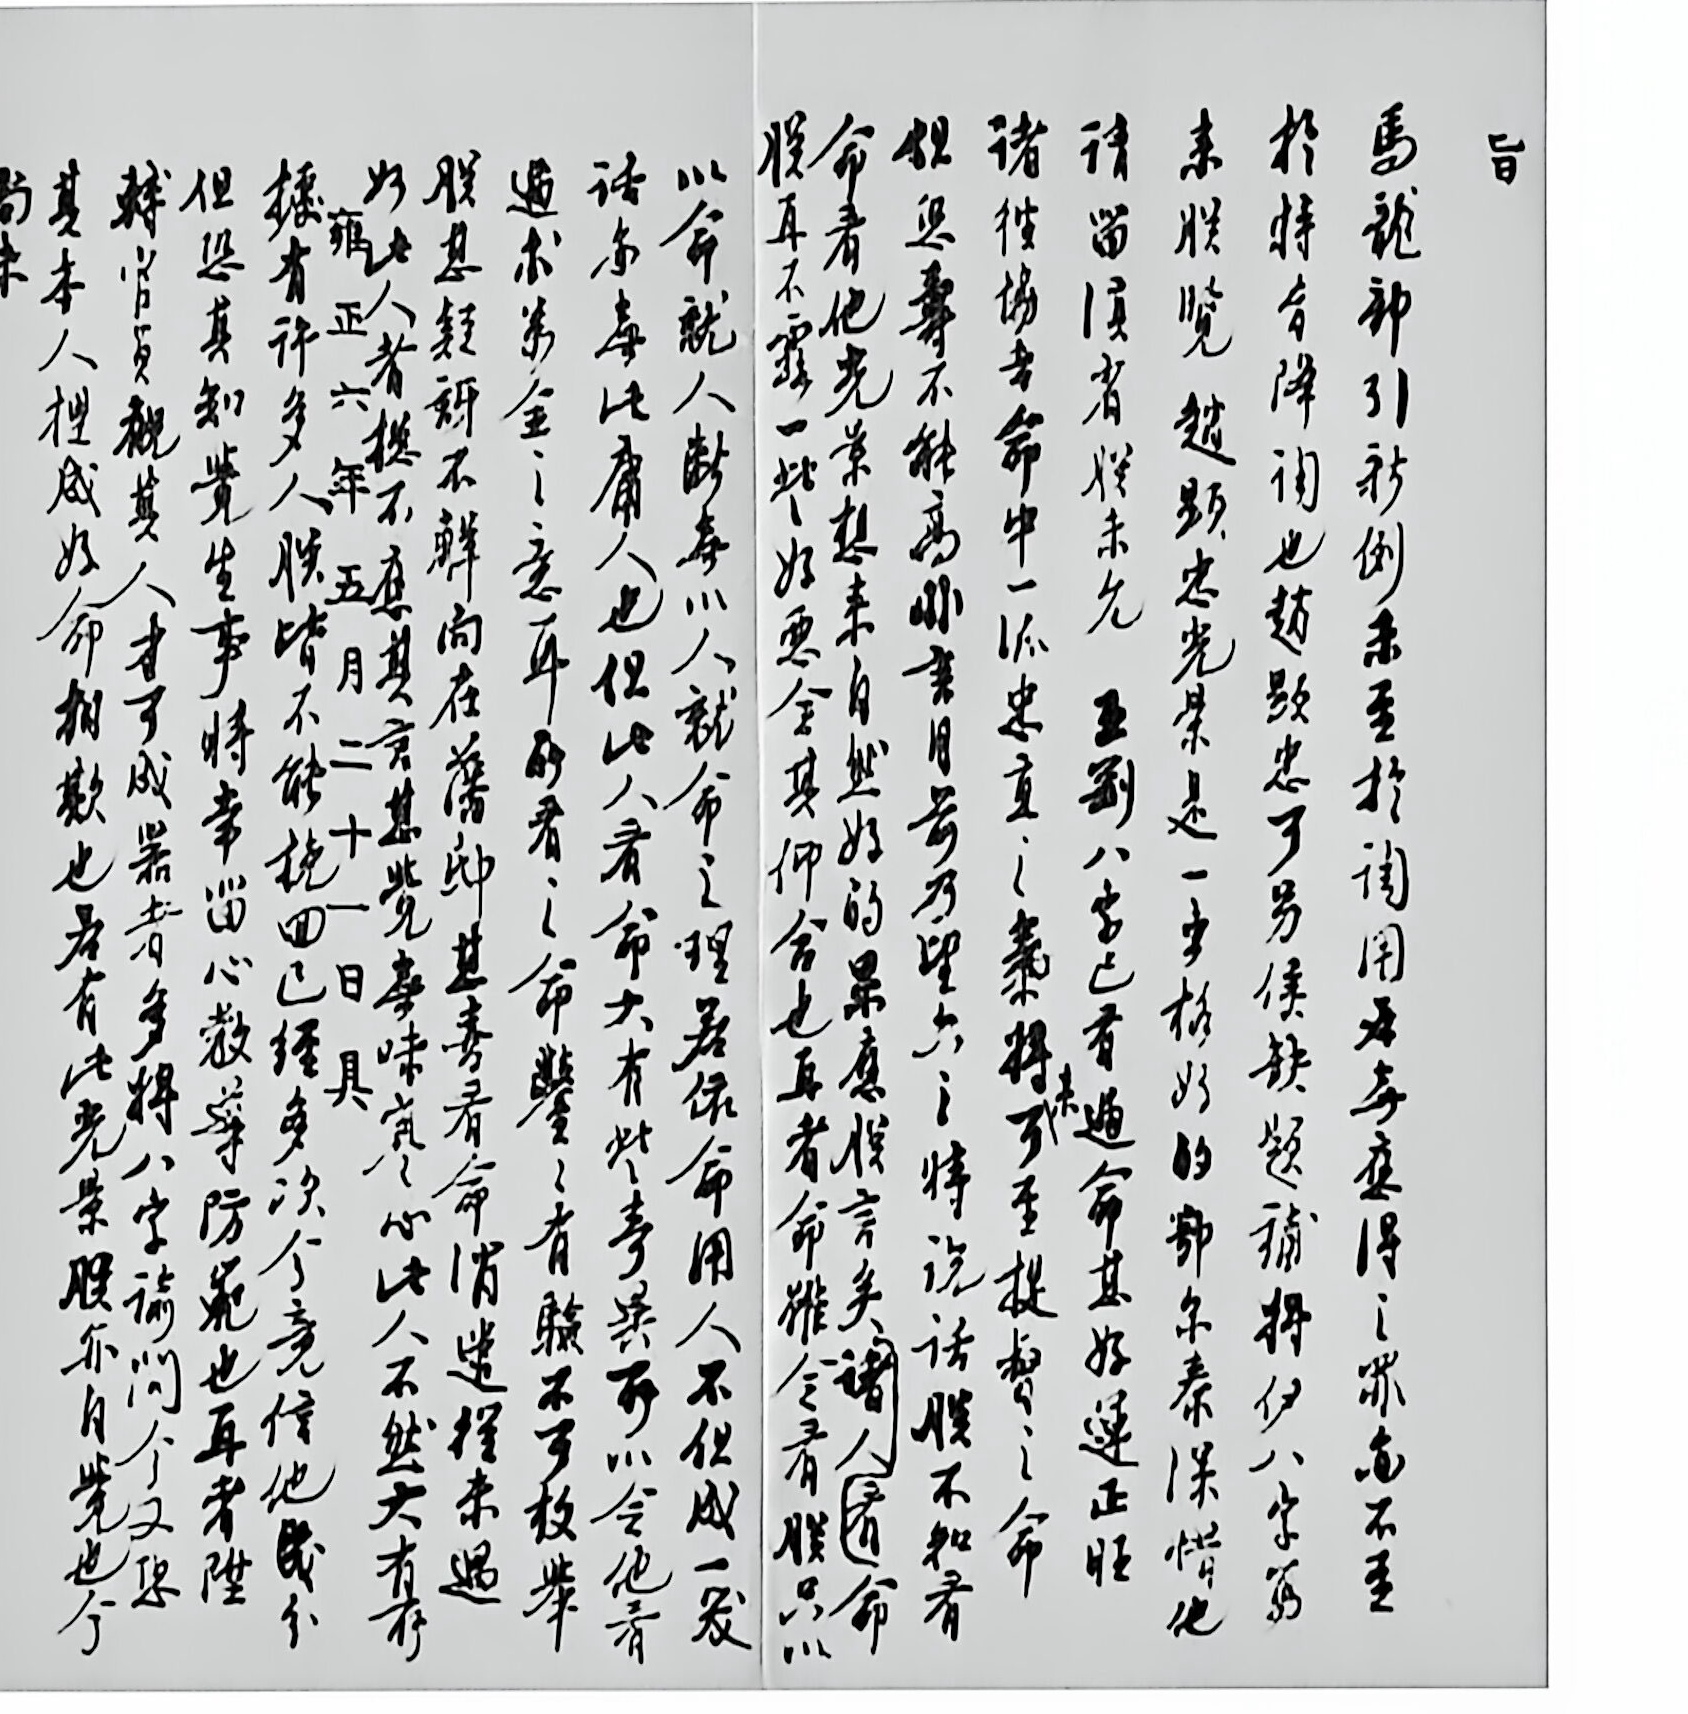
\includegraphics[width=.9\linewidth,height=.68\textheight,keepaspectratio]{assets/fig-100.jpg}
\caption{雍正朱批论八字（于岳锺琪《奏请赵显忠补靖远协副将折》后）。图片与释读文字均来自台北故宫博物院清代档案检索系统，故宫003252号。}\label{fig:100}\end{figure}


% 原书第79页

\begin{bookquote}马龙部引新例，未至于调用，若无应得之罪，亦不至于特旨降调也。赵显忠可另候缺题补，将伊八字写来朕览。赵显忠光景是一出格好的。鄂尔泰深惜他，请留滇省，朕未允。王刚八字已看过，命甚好，运正旺，诸往协吉，命中一派忠直之气。将来可至提督之命，但恐寿不能高。非言目前，乃望六之时说话。朕不知看命，看他光景想来自然好的，果应朕言矣。看诸人命，朕再不露一些好恶，令其仰合也。再者命虽令看，朕只以以命就人，断无以人就命之理，若依命用人，不但成一笑话，亦无此庸人也。但此人看命大有些奇异，所以令他看过，求万全之意耳。所看之命，凿凿有验，不可枚举。朕甚疑讶不解。向在藩邸，甚喜看命消遣，从未遇如此人者，总不应其言，甚觉无味寒心。此人不然，大有所据，有许多人朕皆不能挽回，已经多次，今竟信他几分。但恐其知觉生事，时常留心，教导防范也。再者，升转官员，观其人才可成器者，多将八字谕问，今又恐其本人捏成好命相欺也。若有此光景，朕亦自觉也。今尚未。\end{bookquote}


% 原书第80页

判断某个八字在某个流年的吉凶祸福，重要的一步是看流年的天干与八字中的天干、流年的地支与八字中的地支分别发生了什么作用。在八字算命中，天干与天干之间以及地支与地支之间存在一些固定的公式，会让“天干”或“地支”产生变化，类似于化学反应，让其本身的五行性质发生改变。当流年中的干支与八字中的干支形成特定组合，并符合某些命理推算规则时，这一年中就被认为会出现命运的变化。


% 原书第80页

康熙的八字与这一年的流年戊子就是典型的出现大变化的例子。戊子中的地支“子”，和八字的年支“午”，形成了“子午相冲”；同时“子”字又和月支的“辰”字及日支的“申”字，形成“申子辰三合水”强势组合。用简单直接的话来说，这一年的流年和康熙八字的地支产生了重大反应，改变了命局八字的自有属性和结构。在传统认知中，这样的流年对康熙来说就是有大变化之年。


% 原书第80–81页

至于改变是好是坏，具体印证到什么事情，算命师的水平不一样，解释也不同。解释的部分是主观的，反映了不同测算人的不同水准。但上面提到的天干地支的反应公式是通用的，类似于数学中的“平行线不相交”这样的公理，是所有八字算命流派都需要遵守的基本原理。\NoteRef{03}{19}因而无论使用哪种八字测算流派的方法，都会看到康熙的八字在这一年流年的冲击下出现变化。


% 原书第81页

上面引文中提到太子认为康熙的预测已有应验，康熙回答“尚恐未尽于此”，就是说他认为应验的不止是这件事。这就涉及算命中的第二个问题：应期，就是大概发生在什么时候。比如一个人去算命，说他今年有病灾。那么这个人大病一场后，就会去问算命的，刚得的病是不是已经应了病灾。潜台词就是如果已经应验了，那么今年接下来就平安了。康熙父子间的对话是典型的算命后印证应验时间。至于太子所提到的“一念和尚”的事，六月二十二日有密折告知康熙“一念和尚”已被抓获。\NoteRef{03}{20}由此可知，康熙在这一年的夏天仍然认为预测中的“大事”尚未出现。


% 原书第81–82页

康熙八字的地支与戊子流年的地支之间产生的“子午相冲”与“申子辰三合水”，都指向了八字五行中的水在这一年突然变得很强，形成了克火之势；而与“火”相关的就是康熙八字中出生年份“甲午”中的地支“午”（午的五行属火）。现在遇到的流年“戊子”中的“子”不仅会冲“午”，而且还与月份和日子的地支一起汇合，形成“申子辰三合水”来克“午”火。在这样的情况下，这一年最忌“水”，要小心秋冬之季，因为秋天属“金”，五行中“金”生“水”；而冬天本就属“水”，自然“水”旺。知道了这一点，就可以明白为什么夏天发生了事，康熙会说“尚恐未尽于此”。


% 原书第82页

同时还可以看到，在这一年阴历七月，也就是秋季开始时（废黜太子之前），康熙下谕旨给皇三子和皇四子，命他们二人去安排周围寺庙的喇嘛和和尚，准备大范围念经。康熙这张满文谕旨还存世：


% 原书第82页

\begin{bookquote}（朱谕时间：康熙四十七年七月初六日。）\end{bookquote}

% 原书第82页

\begin{bookquote}八月初一日前七日后七日，着各寺喇嘛尽力诵念《甘珠尔经》。若一寺喇嘛不敷，则令二寺合念。五十喇嘛在中正殿、永宁寺诵经，亦令和尚等在报国寺、广济寺诵经。诵经毕，将各寺诵念数，开明奏闻。\NoteRef{03}{21}\end{bookquote}

% 原书第82页

在接到康熙谕旨后三天即七月初九，皇三子和皇四子联名上奏折表示他们马上去调查各寺庙喇嘛情况，而且还说在研究“如何令和尚在报国寺、广济寺诵经”。《甘珠尔经》是在大事之前祈福所用，但这是一部藏传佛教的经书，因而两位皇子不知道该怎么让汉传佛教的和尚在北京城内的报国寺、广济寺来念。


% 原书第82–83页

五天后即七月十二日，两位皇子禀报康熙，他们已经安排妥当，除了按照康熙的吩咐找了五十六名喇嘛分别在中正殿永宁寺念《甘珠尔经》以外，还找了—


% 原书第83页

\begin{bookquote}广慈寺一百八人、妙英寺七十人、崇国寺一百三十人、慈度寺一百三十人、阿旺扎木苏庙三百人、达赖喇嘛庙八十人、北黄寺一百四十人、敬祝寺八十人尽力诵《甘珠尔经》；永慕寺合裕王庙喇嘛有五十四人，圣化寺加乌思尼哈尚间苏巴尔干喇嘛有五十四人，范景昌加希达达庙喇嘛有五十四人，三佛寺加索诺木绰尔济庙喇嘛有五十四人，令彼尽力诵《甘珠尔经》。雅满达嗄庙有喇嘛二十人，令彼尽力诵蒙古字《甘珠尔经》。再报国寺、广济寺俱置和尚一百八名诵经。\NoteRef{03}{22}\end{bookquote}

% 原书第83页

两位皇子不仅尽力找了众多的喇嘛来念《甘珠尔经》，而且还找了蒙古喇嘛念蒙古文版的《甘珠尔经》。报国寺、广济寺的和尚大概没法念这部经，因而报告中只写了“诵经”。在这份奏报的最后，两位皇子还注明了念经时间按照康熙的吩咐：


% 原书第83–84页

\begin{bookquote}各寺诵经既在八月初一日前七日后七日，则皆本月二十三日起，至八月初八日。\NoteRef{03}{23}\end{bookquote}

% 原书第84页

这一轮经念完后，八月十日康熙又通知两位皇子，让喇嘛再加念七天，从八月十四到二十日。这一次康熙还说到只用喇嘛念，也就是报国寺、广济寺的和尚不用再念经了。\NoteRef{03}{24}


% 原书第84页

《甘珠尔经》是佛陀论说的总汇，在藏传佛教中，诵读这部经有特别的福报。康熙小时候就从孝庄太皇太后那里了解了这部经书的神秘力量。作为虔诚的藏传佛教信徒，孝庄发大愿，集皇家之力，历时两年，使用了黄金、宝石等各种名贵材料制作出了《甘珠尔经》。康熙赐名这套御制《甘珠尔经》的抄本为《龙藏经》，全名为《泥金写本藏文龙藏经》（现存台北故宫博物院，是其镇馆之宝之一）。\NoteRef{03}{25}


% 原书第84页

康熙对《甘珠尔经》的认识来自孝庄，遇到他认为会有危难的时刻，便找喇嘛来诵读这部经。这样大规模安排诵经，在康熙朝并不常见。而且从两位皇子的回奏上看，他们也是第一次这样安排大规模念经，还在摸索如何安排人员，如何分派念经的任务。


% 原书第84–85页

这次念经的时间安排十分特别，八月初一前后七天中并没有什么特别的节日，唯一特别之处就在于那几天正是进入秋天的时节。那年的农历七月二十四日（9月8日）是二十四节气中的“白露”，而念经从七月二十三日开始。“白露”的“白”是代表五行中的“金”，这个节气也意味着秋天的正式开始。康熙选在了秋天开始时来念经，也意味着他知道或者说他相信真正的麻烦事在入秋后才会出现。


% 原书第85页

当然，康熙到底怎么算的命，是他自己算的，还是找人算的，都已经无从知晓。但可以确定的是康熙曾经算过，“有大事发生”这个念头就盘旋在他的脑海里，甚至也在太子的脑海里。对于康熙算命，知道有事发生这一点，连传教士也记录了。


% 原书第85页

在这一年的十二月初一（1709年1月11日），纪理安记载钦天监竟然派人到教堂来为康熙祈福。钦天监这样的朝廷机构到教堂来祈福是很少见的，这也是跟算命有关。纪理安是这样记载的：


% 原书第85页

\begin{bookquote}钦天监再一次为了皇帝的身体健康组织人到我们的教堂来祈祷。七年前他们来过，根据中国的算命术，那一年对皇帝来说，是一个会有重大变化的年份。那一年是马年，跟皇帝的出生年份一样。\NoteRef{03}{26}\end{bookquote}

% 原书第85–86页

跟出生年份一样，就是俗称的本命年。按正常推断，钦天监更多的时候应该是去寺庙念经、去道观做仪式等，只有认为最重大的关键时候，他们才会连教堂都派人去，因而上一次都是七年前的事了。这也从侧面说明，皇帝的命是算过的，而且有专门的机构在做监测。康熙所谓“今岁有事，朕已预知”，并不是未卜先知，而是认真测算后的未雨绸缪。古代算命是日常生活的一部分。皇帝有专门的团队给他定期测算，这和今人定期检查身体健康是差不多的考量。


% 原书第86页

了解康熙一直在琢磨这一年中会有什么大事发生，才能明白当他得知大皇子的镇魇也针对自己时，马上就会相信原来测算中所谓“今岁有事”的实施者不是太子，而是大皇子。他也马上就会认定之前是错怪了太子。根据纪理安记载，康熙在挖出人偶当天，就派太监去宽慰了关押中的太子。纪理安对康熙的心理变化做过分析：


% 原书第86页

\begin{bookquote}（看到挖出来的人偶后）康熙被惊到了；不过他马上松了一口气，意识到喇嘛的法术已经被识破，那也就没有危险了。不过他还是为发生在他和儿子身上的事情感到悲伤。当天，他就派了太监到宫里关押废太子的地方，告诉废太子放宽心，如果真有什么不好的事发生，他的父亲将会和他一起应对。太监还鼓励太子就像以前那样多吃点东西。康熙还下了命令马上恢复太子的待遇，标准和分量都和太子小时候就开始拥有的那些一样。\NoteRef{03}{27}\end{bookquote}

% 原书第86–87页

知道了康熙的心理变化，就明白他为什么会力排众议，坚决要复立太子了：最直接的理由就是他相信之前误会了太子。在复立太子的同时，他也对暗害他和太子的大皇子做出了最严重的惩罚，不仅取消了他所有的封号，还收回了他在八旗内部的人丁和财产。\NoteRef{03}{28}这样相当于在满洲八旗中也消解了大皇子的权势，宣布了他政治生命的死亡。


\begin{sectionnotes}

% 原书注释：原书第396页
\BookNote{03}{1}{Michael D. Bailey, "The Disenchantment of Magic: Spells, Charms, and Superstition in Early European Witchcraft Literature", 383—404.}

% 原书注释：原书第396页
\BookNote{03}{2}{律例解释见薛允升，《唐明律合编》，卷18，459—460。}

% 原书注释：原书第396页
\BookNote{03}{3}{《大清律例》，卷26，“造畜蛊毒杀人”律例下。}

% 原书注释：原书第396页
\BookNote{03}{4}{蔡元培，《〈石头记〉索隐》，10—12。}

% 原书注释：原书第396页
\BookNote{03}{5}{《圣祖仁皇帝实录》，卷234。}

% 原书注释：原书第396页
\BookNote{03}{6}{杨珍，《康熙皇帝一家》，145。关于康熙儿子、女儿的情况，可以参看《康熙皇帝一家》附录中的表格。}

% 原书注释：原书第397页
\BookNote{03}{7}{《圣祖仁皇帝圣训》，卷1。}

% 原书注释：原书第397页
\BookNote{03}{8}{孝惠章皇后对康熙的影响，参看杨珍，《康熙皇帝一家》，第三章。}

% 原书注释：原书第397页
\BookNote{03}{9}{以上一段中所有数据均来自杨珍对《起居注》的统计。详细见杨珍，《康熙皇帝一家》，91—92。}

% 原书注释：原书第397页
\BookNote{03}{10}{《圣祖仁皇帝实录》，卷234。}

% 原书注释：原书第397页
\BookNote{03}{11}{杨珍，《康熙皇帝一家》，65—67。}

% 原书注释：原书第397页
\BookNote{03}{12}{《圣祖仁皇帝实录》，卷234。}

% 原书注释：原书第397页
\BookNote{03}{13}{以上引文均转引自杨珍，《废太子允礽一家与咸安宫》，44。}

% 原书注释：原书第397页
\BookNote{03}{14}{《圣祖仁皇帝实录》，卷234。}

% 原书注释：原书第397页
\BookNote{03}{15}{姚念慈，《康熙盛世与帝王心术》，117。}

% 原书注释：原书第397页
\BookNote{03}{16}{《康熙朝汉文朱批奏折汇编》，册8，813；皇十四子算八字，见《〈文献丛编〉全编》，第3册，141—142。}

% 原书注释：原书第397页
\BookNote{03}{17}{《圣祖仁皇帝实录》，卷82。在档案中，笔者只见到过皇十四子和乾隆的八字，未见到过康熙的八字。现在民间广泛流传带有时辰的康熙八字，笔者无法确认来源，因而未有使用。中国第一历史档案馆李刚在《清代宫廷最有福的女人历史上真实的“甄嬛”》一文中也提到乾隆八字是“目前发现的唯一的清代皇帝八字记载”（页78）。}

% 原书注释：原书第397页
\BookNote{03}{18}{本篇简要分析康熙的八字，以了解其心境为目的，因而不加入其八字在这一时期所处的“大运”这个因素。}

% 原书注释：原书第397页
\BookNote{03}{19}{天干地支的各种互相搭配变化，参看沈孝瞻撰，徐乐吾评注，赵嘉宁注译，《子平真诠评注》，76。}

% 原书注释：原书第398页
\BookNote{03}{20}{《康熙朝满文朱批奏折全译》，582—583。}

% 原书注释：原书第398页
\BookNote{03}{21}{《康熙朝满文朱批奏折全译》，585。}

% 原书注释：原书第398页
\BookNote{03}{22}{《康熙朝满文朱批奏折全译》，585—586。}

% 原书注释：原书第398页
\BookNote{03}{23}{《康熙朝满文朱批奏折全译》，586。}

% 原书注释：原书第398页
\BookNote{03}{24}{《康熙朝满文朱批奏折全译》，596。}

% 原书注释：原书第398页
\BookNote{03}{25}{李保文，《孝庄太皇太后与康熙朝〈泥金写本藏文龙藏经〉》。}

% 原书注释：原书第398页
\BookNote{03}{26}{AP3, 567.}

% 原书注释：原书第398页
\BookNote{03}{27}{AP3, 513.}

% 原书注释：原书第398页
\BookNote{03}{28}{AP3, 521.}

\end{sectionnotes}
\section{众人为什么会一致推举皇八子？}

% 原书第87页

在清朝留下的各种史料中，皇八子都被塑造成中国历史传统中的奸臣形象：结党营私，操弄朝政。比如从《实录》的记载来看，皇八子是夺嫡斗争中最为负面的角色。此处仅少量举出一些康熙废太子后两个月内，《实录》里以康熙口吻写下的对皇八子的评价：


% 原书第87页

\begin{bookquote}八阿哥到处妄博虚名。\end{bookquote}

% 原书第87页

\begin{bookquote}允禩柔奸性成，妄蓄大志，朕素所深知。\end{bookquote}

% 原书第87页

\begin{bookquote}八阿哥允禩，向来奸诈。\end{bookquote}

% 原书第87页

\begin{bookquote}允禩乘间处处沽名，欺诳众人，希冀为皇太子。\end{bookquote}

% 原书第87页

\begin{bookquote}允禩自幼性奸心妄，其纠合党类。\end{bookquote}

% 原书第87页

\begin{bookquote}其母家亦甚微贱。\end{bookquote}

% 原书第87页

\begin{bookquote}允禩素受制于妻……任其嫉妒行恶，是以允禩迄今尚未生子，此皆众阿哥所知者。\NoteRef{03}{29}\end{bookquote}

% 原书第88页

这些评语传递的历史信息是，康熙当着朝臣的面，对皇八子从个人到其母亲与妻子，作了全面否定。事实上从康熙朝《实录》再到雍正朝《实录》，只要涉及皇八子，都保持了这个否定的叙述基调。


% 原书第88页

对于官方历史中大量关于皇八子的恶评，开启夺嫡斗争研究的孟森早已察觉到其中的问题：要是康熙真这样如此反复批评皇八子，为什么群臣又会一致且多次推举皇八子为新太子？这无论如何都不能自圆其说。他认为“斥责允禩”的话，大部分是雍正朝的史官“添入”历史中的。\NoteRef{03}{30}孟森的这一判断在后来的研究中没有得到足够的重视。原因之一是没有其他成系统的材料可供了解皇八子；第二，现有官方历史记载对皇八子的斥责并非漫无章法，而是具有清晰的内在逻辑：众人推举皇八子是因为他们都被皇八子欺骗了。皇八子“奸”，“欺诳众人”，众人才成为了他的党翼。这就可以解释为什么这么多人支持皇八子因为他善于伪装，欺骗了大家。


% 原书第88–89页

这个思路从逻辑上确实能讲通，但是落到现实层面却很难成立。因为支持皇八子的人来自各种背景，要取得全部的支持，不是靠诡计靠权谋就可以的。更何况这种支持还与皇帝的意志相左。比如支持皇八子的老一辈：康熙的舅舅佟国维和康熙的哥哥福全。康熙母亲早亡，他的两个娘舅从小就在他身边。其中佟国纲跟他一起西征准噶尔时战死沙场，剩下的佟国维就成为康熙母家最有名望的人。而康熙的二哥福全也是在朝堂上举足轻重的角色，他是当时努尔哈赤家族除了康熙以外最有地位的人。也就是说康熙母亲以及父亲家族最有发言权的两个人，都推举皇八子。\NoteRef{03}{31}这里要强调一点，后世看到他们对皇八子的举荐，认为他们有可能是为了押宝未来的接班人。但在思考当时人做法时，首先要明白废黜太子是突发之事，当这些朝廷老人在康熙面前推举某某皇子的时候，并不知道未来会有储位之争。像曾在康熙面前赞美皇八子的福全，早在1703年就已经去世。所以这些已经身居朝廷权力顶峰的老人对皇八子的赞美和推荐，应该看作他们对皇八子能力的真心认可。


% 原书第89页

另外，《实录》将大量宗藩贵戚、皇叔皇兄、满族大臣的支持，归结为皇八子结党营私。受传统历史书写的影响，“结党营私”带有贬义。但在清初康熙年间的满人政治生态中，“结党营私”是否全为贬义很值得思考。清朝满人的人力资源就是立足于私人主奴关系的基础上，因而带有很强烈的私性。最明显的例子就是雍正还是皇四子时写给年羹尧的信里，教育他的话：


% 原书第89页

\begin{bookquote}国朝祖宗制度，各王门旗属，主仆称呼，永垂久远，俱有深意。尔狂昧无知，具启称职，出自何典？（见附录四）\end{bookquote}

% 原书第90页

雍正要年羹尧搞明白，满洲祖制就是各个王门之下有自己的人，内部是主仆关系。而年羹尧竟然在署名时用了自己在朝廷的职位，就是把自己视作朝廷的人，把自己当成了公家人，那么雍正就要反问年羹尧，这是“出自何典”？


% 原书第90页

皇四子给在四川做巡抚的年羹尧讲这些话，就是在经营王门之下的私系统。“营私”是满人政治中不可缺少的一部分。他要年羹尧明白他是属于自己王门之下的人，不要忘记了这个身份。那么“结党营私”为什么会被《实录》用作了负面评价？这很可能跟当时编纂《明史》有关。在《明史》中，“结党营私”被视为让明朝最终覆亡的根源，是一个极大的“贬义”词汇。雍正朝编纂《实录》的人，比如张廷玉，正是纂修《明史》之人。但明末和康熙时的情况有很大差别。批判明末“结党营私”的对象是大臣或者太监。而康熙朝书写“结党营私”的对象是皇子，更准确地说，是可能成为新太子的人。在康熙那里，能结党营私，也就是未来的皇帝有能力笼络众人，收复人心，无论从什么角度看都不应该是一种负面的能力。


% 原书第90–91页

对于众人一致支持皇八子，或者是他善于结党营私这个事实，纪理安给出的解释很直接，就是皇八子真的很优秀。纪理安对皇八子有极高的评价，说他是“上帝对朝廷的恩赐”，而且强调说这是“公认”的，还赞美说他几年来“出色的工作让其卓尔不群”。\NoteRef{03}{32}由于皇八子没有负责与传教士相关的差事，纪理安的记录中很少提到他。但在这里，纪理安还是不吝赞美之词。


% 原书第91页

上一章已经写过废黜太子后发生了两桩大案：张明德案和镇魇案。在纪理安的记录中，两案都与皇八子相关。张明德案由皇四子挑起，目标是皇八子；而镇魇案中，大皇子针对的目标是康熙、太子和皇八子。这说明大皇子和皇四子都把皇八子视为皇位的竞争对手，从侧面说明了皇八子在他们心中的分量。


% 原书第91页

前面说到，废立太子这一时期的《实录》只要提到皇八子，往往都附带了负面评论。但有一条记录例外。这一条出现在康熙宣布废黜太子后三天，记载在九月初七庚辰日（10月20日）下面：


% 原书第91页

\begin{bookquote}命贝勒允禩署内务府总管事。\NoteRef{03}{33}\end{bookquote}

% 原书第91–92页

这时的康熙还在回京的路上，而内务府是管理康熙家务事的机构。在即将有大量家务事要处理之时，康熙把这个最重要的职务，跳过了众多年长的皇子，交到了皇八子手中。比较起来，在太子被废后，大皇子和皇四子仅仅被安排去看守废太子，孰轻孰重，一目了然。可见在康熙心中，皇八子确实像纪理安所说的一样优秀，不然也不可能在关键时刻把最重要的职位交给他。


% 原书第92页

废黜太子当天，康熙从行营往京城发了一封密谕，要求皇三子迅速赶来，同时安排皇八子和皇四子留守京城。在这之前，皇三子是留守京城的负责人。由于他与太子交好，因而被康熙调离。这份满文谕旨还存世。学者杨珍注意到这里面的一个重要细节：皇八子的名字放在了皇四子之前。\NoteRef{03}{34}这也就是说皇八子除了被安排管理内务府以外，还在废黜太子后，被任命为管理京城各项事务的总负责人。康熙把这两个关键的位置都交给了皇八子。纪理安在解释皇四子要翻出张明德案来对付皇八子时，给出的理由就是“妒嫉”。\NoteRef{03}{35}


% 原书第92页

由于雍正上台后对皇八子进行政治打压，现存关于皇八子在康熙朝的官方记载十分稀缺，而且内容真假难辨。杨珍通过零散的满文档案还发现，早在废太子案前五年，在处理索额图案的关键时刻，康熙秘密派出的就是皇三子和皇八子。\NoteRef{03}{36}除了太子与索额图有直接联系，自然不适合参与处理以外，康熙选择皇八子其实也是绕过了大皇子和皇四子。也就是说，康熙看重皇八子的才能已经有一段时间了，在废黜太子后选他来处理各种事务，并不是临时起意。


% 原书第92–93页

根据纪理安的记录，张明德案审讯到最后，发现张明德是由皇四子带进皇家圈子的，这也就相当于洗脱了皇八子谋害太子之嫌。纪理安说因为张明德是皇四子带来的，排除了皇八子有行刺太子的可能，因而对皇八子的处罚就降低了。在纪理安的记录中，可以明显看到张明德案对皇八子并没有造成实质性伤害。\NoteRef{03}{37}从这个角度也能解释为什么紧接着的一个月里，群臣还会一致推举皇八子。


% 原书第93页

据《实录》记载，十一月十四日丙戌、十五日丁亥、十六日戊子三天（12月25—27日）康熙和亲近朝臣之间为新太子的人选争论不休。“镇魇”案12月5日结束后，康熙就想要复立废太子，但朝臣们一致选择立皇八子。在12月25日这天，康熙把大臣召到畅春园，告诉大家他“渐觉虚弱，人生难料”，让到场的满汉大臣推选一位皇太子。当时康熙给的谕令是除了大皇子，其他皇子都可以选。满汉大臣分头选择，结果都选了皇八子。他们把选好的结果交给太监，太监再把结果递给康熙。康熙担心结果是在串通下得出，因此在看到结果后，又把投票的满汉大臣全部召到面前，让大家不要互相影响，单独把选择写在纸上，并且让他们回去想一晚上，第二天再来。\NoteRef{03}{38}


% 原书第93–94页

第二天（12月26日，丁亥日），康熙在众人投票前，先讲了孝庄太皇太后几次在他用兵的关键时刻给他托梦的往事，然后强调最近又梦到了孝庄太皇太后，对他废黜太子之事表示了不悦。同时，他还说梦到了皇后，也就是废太子的生母。最后他讲到了废黜太子前后的各种奇异之事，并认定那些事都是镇魇所致。总结起来，康熙的开场白明确表达了他想要复立太子的意愿，但群臣还是选了皇八子。《实录》中第三天，康熙再次召众臣前来商议。这次一开场，康熙就讲了很多废太子以前的好事，再次明确指出之前出现的问题都是镇魇所致。最重要的是，当天康熙还把废太子带来了，给了他一个机会，让他当着大臣们做了一个自我陈述。最后，康熙正式宣布释放废太子。\NoteRef{03}{39}


% 原书第94页

康熙这三天与众人的争执，《实录》记载得十分详细，总共有约两千五百字。纪理安的《北京纪事》中也详细记录了这几天的争论。大体来说，《北京纪事》的记录与康熙朝《实录》一致：群臣推举皇八子；经过几轮争议依然没有结果；最后没有确立新太子。很明显，这次争论的核心问题在于康熙如何给出他不选皇八子的理由。对于这个问题，《北京纪事》给出了和《实录》完全不同的说法。


\begin{sectionnotes}

% 原书注释：原书第398页
\BookNote{03}{29}{以上诸条出自《圣祖仁皇帝实录》，卷234—235。}

% 原书注释：原书第398页
\BookNote{03}{30}{孟森，《明清史讲义》，467—468。}

% 原书注释：原书第398页
\BookNote{03}{31}{杨珍，《清朝皇位继承制度》，217。}

% 原书注释：原书第398页
\BookNote{03}{32}{AP3, 484.}

% 原书注释：原书第398页
\BookNote{03}{33}{《圣祖仁皇帝实录》，卷234。}

% 原书注释：原书第398页
\BookNote{03}{34}{杨珍，《关于满文档案与清史研究的几点认识》，214。}

% 原书注释：原书第398页
\BookNote{03}{35}{AP3, 484.}

% 原书注释：原书第398页
\BookNote{03}{36}{杨珍，《关于满文档案与清史研究的几点认识》，214。}

% 原书注释：原书第398页
\BookNote{03}{37}{AP3, 484.}

% 原书注释：原书第398页
\BookNote{03}{38}{《圣祖仁皇帝实录》，卷235。}

% 原书注释：原书第398页
\BookNote{03}{39}{《圣祖仁皇帝实录》，卷235。}

\end{sectionnotes}
\section{康熙为什么不选皇八子？}

% 原书第94页

完全出乎康熙的意料，12月25日他召集的满汉诸臣投票，竟然全部投给了皇八子，这个结果让想要复立太子的康熙十分为难。根据《实录》的记载，他让众臣再作考虑，并给出了他不选皇八子的理由：


% 原书第95页

\begin{bookquote}八阿哥未尝更事，近又罹罪，且其母家，亦甚微贱。尔等其再思之。\NoteRef{03}{40}\end{bookquote}

% 原书第95页

前面已经提到，《实录》在康熙废立太子这一时期密集写入的大量康熙批评皇八子的话，都应该仔细推敲。比如这句话的开头，康熙说八阿哥“未尝更事”一句就十分可疑。康熙前不久才让皇八子负责北京的内外事务，又怎么会说他还未更事？此时皇八子二十八岁，皇三子三十二岁，皇四子三十一岁，皇子间的年龄差别其实不大，不存在“未尝更事”这样的情况。“近又罹罪”显然指的是张明德案。但这个案子已在朝廷内外公认是无关大局之事。就连康熙自己也在十天后（1709年1月8日）就“复封允禩为多罗贝勒”\NoteRef{03}{41}。所以很难相信康熙会用自己都不相信的理由来堵众人之口。《实录》中涉及皇八子的评论，许多都难以自圆其说，这也是历代清史研究者都注意到的问题。


% 原书第95页

在25号选新太子的前两天，纪理安的记录提到，他和巴多明神父在宫里碰到一辆镶着金边且用黑布罩着的马车。他们上前询问当差的人，才知道里面坐的是废太子，准备前往畅春园。康熙这时已经在准备让太子与朝臣见面了。\NoteRef{03}{42}


% 原书第95–96页

12月26日，纪理安简单记录了众臣对于皇八子的选择。12月27日，纪理安再次记录了康熙与众臣未能达成一致。在记录朝廷之事以前，纪理安交代了他这一次的消息来源—康熙身边的奴才赵昌。他之所以能从赵昌处探得消息，是因为12月24日徐日昇神父去世。12月26日，康熙传话给京中传教士，让他们再推举一位神父来顶替徐日昇的位置，负责代表众传教士与康熙联系。12月27日，赵昌把所有传教士集中到一起，告诉他们，康熙看了众多传教士的推举后，决定由纪理安、巴多明和苏霖三位神父共同接替徐日昇的位置，都是联系人。宣布完正事以后，赵昌给传教士们讲起了在畅春园里康熙与众臣关于新太子人选的争论。


% 原书第96页

赵昌是谁？为什么纪理安要专门提到他？他提供的信息有多大分量？赵昌比康熙小三岁，作为康熙的包衣奴才，从小就跟在康熙身边，陪伴康熙。在满人传统中，这种年少时就跟随陪伴在主子身边的奴才叫“哈哈珠子”，类似于中国传统中的伴读、书童。但是满人的陪伴不只是读书，还有骑马、射箭这些活动。赵昌长大后，较长时间担任的是养心殿监造和侍卫。他是活跃在内廷中长期为康熙所亲近的奴才。\NoteRef{03}{43}纪理安提到赵昌，意在说明他记录的并不是坊间的小道消息。


% 原书第96页

赵昌给传教士讲了满汉大臣分别用满文和汉文写投票，结果所有的票都投给了皇八子。这一点和《实录》的记载一致。但赵昌还讲到了为什么康熙否定了众人提议的皇八子，这个答案就和《实录》所给出的完全不一样了。赵昌说康熙的理由是


% 原书第97页

\begin{bookquote}皇八子肯定是很有天赋的，但是从行军打仗的要求上说，他不够强硬。\NoteRef{03}{44}\end{bookquote}

% 原书第97页

也就是说，康熙给的理由是皇八子的“武”不行。这和《实录》中的“八阿哥未尝更事，近又罹罪，且其母家，亦甚微贱”完全是两个意思。


% 原书第97页

两相对比，很明显《北京纪事》中所言皇八子“武”不行，是一个可以服众，同时也符合满人传统的理由。在清朝初年的满人世界中，“武”是比“文”更被看重的素质。那为什么雍正朝的史官把皇八子“武”不行省略掉，而换上其他的缺点呢？这是第七章主要探索的问题，也是理解康熙晚年选择太子标准的重要线索。


\begin{sectionnotes}

% 原书注释：原书第398页
\BookNote{03}{40}{《圣祖仁皇帝实录》，卷235。}

% 原书注释：原书第398页
\BookNote{03}{41}{《圣祖仁皇帝实录》，卷235。}

% 原书注释：原书第398页
\BookNote{03}{42}{AP3, 542.}

% 原书注释：原书第399页
\BookNote{03}{43}{关于赵昌的研究，参看陈国栋，《康熙小臣养心殿总监造赵昌生平小考》。}

% 原书注释：原书第399页
\BookNote{03}{44}{AP3,549.}

\end{sectionnotes}
\section{群臣为什么不愿意复立太子？}

% 原书第97页

《实录》和《北京纪事》都记录了康熙向众人表达过复立太子的愿望，也都明确写出了众人在听了康熙的选择后，仍然坚持要选皇八子。为什么群臣如此坚持？《实录》没有回答这个问题，而是塑造出一个奸猾、结党的皇八子形象，所以后世顺着这个思路作出的解释是，众人都被皇八子蒙蔽了，因而与他结党。\NoteRef{03}{45}


% 原书第98页

《北京纪事》对群臣拒绝复立太子给出了一个与传统理解完全不一样的逻辑。这个逻辑的起点是这一时期康熙病重，而且到了随时有可能去世的地步。康熙进入12月以后出现严重的心悸问题，让他很难受。症状是晚上心跳加速到无法入睡。康熙用了各种中医调理，都没有效果。无奈之下，他找到了传教士，让他们商议给出治疗方案。鉴于不久前治疗皇十八子失败，传教士群体这时对开药十分谨慎。经过众议，他们最后给出的方案是用红酒送服酊剂阿尔格而墨斯（tincture of arkemes）。这一药物是在地中海地区广泛使用过数百年的日用饮品的提纯版，安全性有保证，好几位传教士自己都吃过。\NoteRef{03}{46}


% 原书第98页

对于康熙这段时间的病，《实录》没有明确记载，但当时皇帝病重是官场上广为人知的。在满文和汉文奏折中，有许多跟康熙亲近的地方官都在问询康熙的身体健康。山西巡抚的满文奏折中说他12月（阴历十一月）先后去五台山、恒山，给康熙烧香祈福（不是康熙安排的，而是他自愿去的）。康熙回文给他说：“今较前好些，但还很弱。”山西巡抚回复中写到“奴才昼夜焦虑”，准备“洁身斋戒”来为康熙祈福。\NoteRef{03}{47}陕西巡抚、川陕总督、甘肃巡抚都在上奏折问安。汉文奏折中还可以看到直隶总督、陕甘总兵上奏折关心康熙的身体健康。\NoteRef{03}{48}从这些奏折中可以看到，康熙的病和传教士记录的症状一致：


% 原书第99页

\begin{bookquote}……朕体渐弱，心跳加增甚重。\NoteRef{03}{49}\end{bookquote}

% 原书第99页

\begin{bookquote}……伏知圣躬或夜心跳，寝息稍有不安，故奴才不胜焦虑。\NoteRef{03}{50}\end{bookquote}

% 原书第99页

而且康熙在多封奏折的批复中都表示自己很虚弱。在一封给川陕总督的朱批中，甚至写到“朕今仍不能写”\NoteRef{03}{51}。由于太虚弱，写字都很吃力了。


% 原书第99页

有了这个重病的背景，才能理解当时群臣在选择新太子时的心境。他们并不知道康熙这次能不能挺过去，所以当时考虑的并不仅仅是立一位很多年后才会登位的新太子，而是在选有可能马上成为新皇帝的人。其次，还要设身处地站在群臣的角度思考，很多人在太子被废后就迅速更换了门庭。两个月前康熙废太子时以很坚决的方式拒绝任何说情，因而绝大部分臣子都没有预料到，如此决绝废掉的太子还会被复立。


% 原书第99–100页

我们作为后来人，当然知道康熙朝后面还有很多储位之争的故事，但当时的人无法预知。立了三十几年的太子被废，京城大小官员在震惊之余，马上会思考的问题就是：接下来怎么办？谁会是未来的太子？而皇八子，一是能力有目共睹，二是康熙刚废太子后，就把管理内务府和京城事宜交给了他，这些都注定了在废黜太子后，各路人马会聚集到皇八子处。10月17号宣布废黜太子，京城中的各种势力不会按捺两个月都没有动静，直等到12月25日康熙让他们推举人选的时候才开始思考未来新主的问题。皇八子府上早就门庭若市，应该是一个合理的推测。在这种情况下，有的人落井下石，有的人改换门庭，各种世态炎凉、人情冷暖的故事也大概率已经围绕着太子和皇八子展开。


% 原书第100页

当12月25日，满汉诸臣第一次统一推举了皇八子后，他们就已经公开做出了政治选择。康熙这时候再给他们讲皇八子的不足，他们能怎么选择？站在当时选了皇八子的众臣角度来思考，他们已经没有办法再改变他们的决定了。他们选择皇八子已经深深伤害和得罪了太子。这是既成事实。大家这时都害怕太子复位。特别是当时康熙身体也不好，众臣在选择的是有可能马上上台的新皇帝。康熙自己也明白马齐等人选皇八子已经宣告了与太子之间的关系破裂，用康熙的话说，马齐等人“皆系已与皇太子反目之人”\NoteRef{03}{52}。


% 原书第100–101页

从纪理安的记录中可以看出，康熙已经觉察到了群臣的这一担忧，因而他把众臣召集起来，让太子给他们讲话。对于讲话的内容，纪理安强调的点是太子向大家保证他不会报复。康熙也强调了这一点。纪理安解释，这时大家的态度变成了请康熙自己定夺新太子的人选。也就是说，康熙要立谁，是他自己的事，但是群臣不愿意改变他们的选择。纪理安还写到，根据他所了解的情况，大臣之间已经互相达成了一致。他们认为应该让皇帝自己决定要选谁当太子，而不是由他们出来支持复立太子。纪理安还专门强调，就是那些之前反对废黜太子的人，也认为应该这样。\NoteRef{03}{53}


% 原书第101页

李光地记录在四十八年正月（1709年2月）期间，康熙曾单独责问他：“去秋卿言云何？而今乃遽改口，与众同声耶？”在上一章已经讲过，李光地对康熙废太子持反对意见，还反问过康熙，因而现在康熙责问他为什么改口了，和众人一个腔调，不拥护太子了。李光地的回答是：“建储大事也，义当决自圣衷。”\NoteRef{03}{54}这个回答和纪理安的分析完全相合，就是大臣们认为，立谁为太子应该由康熙自己决定。


% 原书第101页

1708年12月25日，即开始商讨太子人选的第一天，宫里曾专门派太监和内务府的人来通知传教士，康熙吃了他们开的药后觉得有效。\NoteRef{03}{55}同时，康熙也下令让两广总督到广州西洋人那里找寻药的原材料。\NoteRef{03}{56}由于康熙吃了药后身体见好，在与众人就未来太子人选不能达成一致的时候，便推迟了新太子选举。在新太子人选无着的情况下，12月27日康熙正式释放了废太子。


% 原书第101–102页

在这一天释放太子是《实录》和《北京纪事》共同记录的内容。《北京纪事》还记录了一条一直困扰着清史研究的问题：皇十三子为什么从这一段时期的史料中消失了？到底发生了什么？《实录》记载了秋天皇十三子跟着康熙、大皇子、太子等一起外出。途中太子被废，其他几位成年皇子在清史中也都有交代，唯独对皇十三子这个成年皇子没有提及。皇十三子在皇四子继位后成为重要人物，这是众所周知的。纪理安在写完释放太子后，顺带写了一句：


% 原书第102页

\begin{bookquote}（宣布释放废太子）同时，他（注：康熙）还恢复了皇十三子，和太子的两个儿子，也就是他的孙子的自由。\NoteRef{03}{57}\end{bookquote}

% 原书第102页

根据这条记录，皇十三子在外出狩猎时，很可能与废太子行事有关联，因而也被关了起来。皇十三子在雍正时期成为了最重要的王爷，对他不利的历史，应该都被雍正朝的史官们删除了。到底他犯了什么事，也许永远都是一个谜。


\begin{sectionnotes}

% 原书注释：原书第399页
\BookNote{03}{45}{康熙因为皇八子结党而对其有意见是目前学界主流认识：孟森，《明清史讲义》，467—468；杨珍，《清朝皇位继承制度》，222—223。}

% 原书注释：原书第399页
\BookNote{03}{46}{传教士分析康熙的病情时，用了英国医生哈维（1578—1657）发现的人体血液循环理论来解释他心悸的原因。对于这次治疗的大概情况，有传教士写信回欧洲时说起，还有相关的研究。参看《耶稣会士中国书简集—中国回忆录》，卷2，殷弘绪37；董少新，《形神之间：早期西洋医学入华史稿》，113；关雪玲，《康熙时期西洋医学在清宫中传播问题的再考察》，143—145。以前学者对康熙到底吃的什么药有争议，因为他在吃了药后还发了汉文谕旨给两广总督，让他找药，汉文谕旨：“着寻西洋格而墨斯，着实要紧……如无，将阿尔格而墨斯速速送来。”（《康熙朝汉文朱批奏折汇编》，册2，299—300）。这里提到“格而墨斯”与“阿尔格而墨斯”是两样东西。同时这段历史在江西的殷弘绪神父信中（《耶稣会士中国书简集》）提到，其中治疗康熙的药物在翻译成中文时写的是“胭脂红酒”。“格而墨斯”、“阿尔格而墨斯”与“胭脂红酒”互相有什么关系是学界尚未厘清的问题。“格而墨斯”（kermes）很多地方翻译为胭脂，因其是从昆虫躯体中提取的一种古老的朱红色颜料。同时格而墨斯也是制作“阿尔格而墨斯”（arkemes）的主要原料。“阿尔格而墨斯”是一种意大利药用饮料，很早就用来治疗心悸等病，现在依然有卖。《耶稣会士中国书简集》中的“胭脂红酒”并不是第三种东西。经查《耶稣会士中国书简集》法文底本（Lyon本，v10，53），殷弘绪就是写的arkemes，而翻译者将其意译成了“胭脂红酒”。根据纪理安的记录，康熙治疗所需的是酊剂的阿尔格而墨斯（tincture of arkemes,用乙醇提取的浓缩品）。康熙的宫中和北京的教堂中，都有专门的实验室，他们有能力做药物提取与合成。所以康熙给两广总督的谕旨中会要求首选“格而墨斯（kermes）”这个原料，如果找不到，那么再要已经合成过的“阿尔格而墨斯（arkemes）”。Arkemes是商品，当时被广泛使用，因而康熙和北京的传教士知道arkemes在广州的西洋人那里容易找到，反而是作为原材料的kermes可能一时难以找到。对于酊剂的阿尔格而墨斯，当时传教士嘱咐康熙用红酒送服，所以才有之后康熙通知沿海官员给他寻找红酒。}

% 原书注释：原书第400页
\BookNote{03}{47}{《康熙朝满文朱批奏折全译》，609—610。}

% 原书注释：原书第400页
\BookNote{03}{48}{《康熙朝汉文朱批奏折汇编》，册2，267—275。}

% 原书注释：原书第400页
\BookNote{03}{49}{《康熙朝满文朱批奏折全译》，606。}

% 原书注释：原书第400页
\BookNote{03}{50}{《康熙朝满文朱批奏折全译》，606。}

% 原书注释：原书第400页
\BookNote{03}{51}{《康熙朝满文朱批奏折全译》，606。}

% 原书注释：原书第400页
\BookNote{03}{52}{《康熙朝满文朱批奏折全译》，1653。}

% 原书注释：原书第400页
\BookNote{03}{53}{AP3,544-545.}

% 原书注释：原书第400页
\BookNote{03}{54}{《李文贞公年谱》，197。}

% 原书注释：原书第400页
\BookNote{03}{55}{AP3,543.}

% 原书注释：原书第401页
\BookNote{03}{56}{《康熙朝汉文朱批奏折汇编》，册2，299—300。}

% 原书注释：原书第401页
\BookNote{03}{57}{AP3, 549.}

\end{sectionnotes}
\section{君臣拉锯}

% 原书第102–103页

到1708年12月27日止，《实录》和《北京纪事》的记录中都能反映出康熙复立太子的愿望很强烈。但《实录》一直到四十八年正月二十一日癸巳（1709年3月2日）才再次出现与立太子事相关的记录。凭常理推断，12月27日康熙和群臣还在紧急筹商立太子的大事，不大可能突然就停止了，而且一停就是两个多月。


% 原书第103页

纪理安的记录正好为我们提供了这关键的两个月中的大事梗概。原来，康熙在一月之内又数次向大臣们表达了复立太子的意思。在1月24日的记录中，纪理安说大臣们还是坚持选皇八子。他特别提到了一位姓马的阁老向康熙汇报说，内阁中满汉大臣都坚持推举皇八子，康熙很生气，于是赌气说自己身体还好，太子就先不选了。这位姓马的阁老就是马齐。


% 原书第103页

纪理安接下来便讲到了清史中一个富有争议的桥段：殴曳马齐。这件事情是否真的发生过？纪理安说因为马齐等人坚持推举皇八子，康熙为了反驳马齐，给他讲了很多道理，越说越生气，于是“一拳把马齐打倒在地”，然后马齐还倒在地上的时候，便被人拖了出去。\NoteRef{03}{58}纪理安的记录完全对上了《朝鲜实录》中的“殴”和“曳”这两个动作。纪理安在写完这一场景后，还写到第二天有二十位高官以年龄和身体原因请辞。群臣用这样的方式对康熙的所为作出了抗议。\NoteRef{03}{59}


% 原书第103页

纪理安认为“殴曳马齐”涉及君臣间的博弈，为此他有过一段分析：


% 原书第103–104页

\begin{bookquote}尽管他们知道皇帝有意复立太子，他们还是报告说应该选择皇八子。大臣们这样建议并不是他们怀疑皇帝真的想要复立太子，而是他们想要告诉皇帝他在如此重大的问题上（注：指废黜太子）仓促行事已经带来了很大伤害，同时也是让皇帝知道他今后应该习惯于先把大臣召来听了他们的意见后，再做决定。\NoteRef{03}{60}\end{bookquote}

% 原书第104页

康熙在巡行路上，尚未回到北京时，就匆忙宣布了废黜太子。纪理安分析康熙的一个考虑就是为了避开朝臣的反对。回京以后，康熙又在很长一段时间内拒见任何官员，也是为了避免朝臣的谏言。\NoteRef{03}{61}所以在传教士看来，北京官员集团是在借太子问题反对康熙不尊重朝廷制度，以及康熙在太子问题上的朝令夕改。


% 原书第104–105页

高官集体上辞呈，这是君臣关系中朝臣表达抗议的手段。传教士没有记录康熙如何应对辞呈，但传教士记录了两件事，可以看出康熙决心对抗群臣。一是1月27日在一位公主出嫁的宴会上，康熙安排在正厅的显著位置放置了三个座位：一个是他自己的，一是给皇太后的，还有一个是给废太子的。康熙通过这样的安排来重塑废太子的地位。\NoteRef{03}{62}第二件事是康熙取消了新年当天与文武官员的筵宴来对抗群臣。同时，纪理安提到康熙这样行事只是针对大臣。因为新年前三天（2月7日），传教士获允进宫给康熙请安，康熙还是像往年一样给传教士派发了礼物。第二天，传教士又再次进宫感谢康熙的恩赐。\NoteRef{03}{63}康熙这一年新年没有参与筵宴，在《实录》中有所提及。但只有看了传教士的记录，才知道他没有参加的原因。


% 原书第105页

出乎康熙意料的是，康熙新年拒见文武百官，被坊间理解为他已病危。为此，康熙在2月13日那天亲自现身北京城辟谣。纪理安解释，按照惯例，皇帝经过的地方要提前清跸道路，各个路口都有士兵把守，沿途的商店也要关闭。但为了破除谣言，康熙要求不得关店和提前封路。他带了六个太监，骑着马从宫里出来，在百姓的注目下，前往畅春园。这样一来，谣言不攻自破。\NoteRef{03}{64}从传教士的记录中可以看到，整个1709年的1月和2月，康熙都在用各种方法表达他坚持要复立太子的决心。


% 原书第105页

康熙在康熙四十八年三月初九日（庚辰日，1709年4月18日）宣布复立太子。新年过后到太子复立的这段时间内，《实录》于四十八年正月二十一日（1709年3月2日）和二十二日（3月3日）之下，又长篇记录了康熙与大臣们就新太子人选的争执。这两天的记录是以康熙与朝臣对话的形式呈现的。这时领头支持皇八子的人有两位：马齐和康熙的舅舅佟国维。这两天的内容总结起来就是：众臣还是坚持选皇八子。同时马齐被康熙认为是带头人，因而康熙传令把马齐和他的兄弟都革职关了起来。


% 原书第105–106页

单独看《实录》的记载会有一个疑问，从3月3日康熙与群臣的争吵到4月18日太子复立这一个多月里发生了什么？整个局面是如何扭转的？这些问题在《实录》中都没有答案。而在这期间，《北京纪事》首先记载了康熙的身体在吃了传教士开的药以后，慢慢好转。康熙还专门召见了全部传教士，并且下发了公文让朝廷上下知道他的身体在传教士的药物帮助下恢复了。康熙这一时期已经开始外出打猎，开始了各种春天的活动。《北京纪事》是在4月20日（复给太子册宝后一天）下记录的复立太子。


% 原书第106页

《北京纪事》记录了康熙在得不到群臣支持下想到的办法：他决定不争取复立太子，而是取消之前废黜太子的决定，而取消废黜太子的原因是基于太子之前是在巫术的控制下生病了。现在病好了，这个原因没有了，当然也就应该取消废黜太子的决定。\NoteRef{03}{65}尽管最后群臣也并没有让步，但康熙自己找到了一个能昭告天下的理由。


% 原书第106页

无论废黜还是复立太子，康熙都“昭告天下”，那普通士人和老百姓的反应又是什么呢？尽管由于士人文集中对这次废立鲜有记载，更难了解民间对这次废立的反应，但有一点应该是可以确定的，就是当时针对这件事是有民意的。本书前言中提到过清初名士朱彝尊在听闻太子复立后，写下了一首《三月十日诏下青宫再建喜而赋诗》的五言律诗。江西的殷弘绪神父在一封发回欧洲的信中，也讲到了太子废立。在说到太子被复立时，他写道：


% 原书第107页

\begin{bookquote}太子遂依帝国惯常礼仪复位。人们到处显得兴高采烈，有人还据与新发生的一切颇为相似的一段历史往事编了一部戏，且上演至今。\NoteRef{03}{66}\end{bookquote}

% 原书第107页

当然，在《实录》等所有的官方历史书写中，都看不到这里所谓的“喜”。根据历史编写的需要，最后天命是要归在皇四子身上，因而对于“复立”也就无“喜”可言。


% 原书第107页

康熙朝《实录》是雍正朝编订的。这部最重要的记录康熙朝历史的官方编年史书需要体现出合理的历史大势。这个大势就是其他皇子各有各的毛病，都不适合做皇帝。大皇子、太子、皇三子、皇八子、皇十四子在《实录》中出现时，都有这样那样的负面评论。唯一的例外是皇四子，他的名字每次出现都伴随着正面评价。这一正面形象的树立，应该是《实录》编订时的一个重要目标。而这个目标是如何通过删减与虚构来实现的？这是下一章要回答的问题。


\begin{sectionnotes}

% 原书注释：原书第401页
\BookNote{03}{58}{AP3, 585–586.}

% 原书注释：原书第401页
\BookNote{03}{59}{AP3, 586.}

% 原书注释：原书第401页
\BookNote{03}{60}{AP3,543-545.}

% 原书注释：原书第401页
\BookNote{03}{61}{AP3, 480–481.}

% 原书注释：原书第401页
\BookNote{03}{62}{AP3, 586.}

% 原书注释：原书第401页
\BookNote{03}{63}{AP3,593-594.}

% 原书注释：原书第401页
\BookNote{03}{64}{AP3, 598.}

% 原书注释：原书第401页
\BookNote{03}{65}{1709 年 4 月 20 日条目下，Acta Pekinensia, in the Roman Archives of the Society of Jesus, Jap. Sin. 138, 1177–1178。感谢Paul Rule 教授（1934—2024）为我提供该资料。}

% 原书注释：原书第401页
\BookNote{03}{66}{《耶稣会士中国书简集》，卷2，36。}

\end{sectionnotes}
